% !TeX root=../main.tex
\chapter{آشنایی با ابزار‌های توسعه}
در تمام ابزارهای ذکر شده در ادامه این متن حتما باید به ورژن هر کدام دقت شود،
ورژن‌ها باید با یکدیگر همخوانی داشته باشند در غیر این صورت مشکلاتی در
کامپایل و اجرای برنامه به وجود می‌آید که به راحتی قابل رفع کردن نیستند.
در انجام این پروژه عدم همخوانی ورژن‌های مختلف ابزارها با یکدیگر باعث ایجاد مشکلات فراوانی شد،
به همین دلیل ورژن مورد نیاز هر ابزار در توضیحات پروژه در گیت‌هاب ذکر شده است.
لیست کاملی از این ابزارها با جزئیات بیشتر را میتوان در کتاب
\lr{Mastering Ethereum}\cite{MasteringEthereum}
در ضمیمه
\lr{D}
مشاهده کرد.

% ------------ Section 3.1
\section{ابزارهای ساده}
\begin{itemize}
	\item \textbf{ویرایشگر}\\
	برای برنامه نویسی این قرارداد هوشمند از ویرایشگر
	\lr{VSCode}
	با نصب پلاگین مربوط به سالیدیتی
\LTRfootnote{https://marketplace.visualstudio.com/items?itemName=JuanBlanco.solidity}
استفاده شده است.
این پلاگین با یافتن اشتباه‌ها پیش از کامپایل و راهنمایی در نوشتن کد قرارداد
کمک شایانی به افزایش سرعت توسعه می‌کند.

	\item \textbf{ورژن‌کنترل}\\
	این پروژه از روز نخست به صورت متن‌باز توسعه یافته است،
	برای توسعه یک پروژه به صورت متن‌باز اولین ابزار مورد نیاز یک برنامه ورژن کنترل است
	که نسخه‌های متفاوت و تغییر یافته کدها را به صورت مرتب نگهداری کند.
	برای این منظور از گیت‌هاب
	\LTRfootnote{\url{https://github.com/}}
	استفاده شده است.

	\item \textbf{بسته‌های Node و NPM}\\
از آنجایی که کدهای سالیدیتی در واقع جاوا‌اسکریپت هستند،
به ابزارهای توسعه اپلیکیشن‌های جاوااسکریپت برای توسعه سالیدیتی نیاز است. ابزارهایی مانند
\lr{Node}
برای کامپایل کردن برنامه‌های جاوااسکریپت و
\lr{NPM}
که مدیریت بسته‌های جاوااسکریپتی که نصب می‌شود را به عهده دارد.

\end{itemize}


% ------------ Section 3.2
\section{کیف پول \gls{Metamask}}
کیف پول دیجیتال متامسک از پرکاربردترین کیف پول‌ها
برای ارتباط برقرار کردن با اپلیکیشن‌های غیرمتمرکز است.
کاپو نیز برای امضای تراکنش‌ها و ایجاد ارتباط با شبکه بلاکچین از کیف پول متامسک استفاده می‌کند.
برای انجام صحیح این عملیات کاربر باید از پیش کیف پول متامسک را نصب کرده باشد و سپس با انتخاب گزینه
\lr{Connect Wallet}،
کاپو درخواست اتصال به کیف پول و دریافت آدرس کاربر را به متامسک ارسال می‌کند.
متامسک نیز پس از دریافت درخواست کاپو از کاربر اجازه اتصال به برنامه را می‌گیرد.
در صورت تایید کاربر آدرس کیف پول به کاپو داده می‌شود.

از این پس هرگاه که کاربر بخواهد در کاپو تراکنشی از جمله
ساخت توکن جدید یا انتقال یک توکن به آدرس دیگر را انجام دهد،
کاپو از متامسک درخواست می‌کند که با
\gls{Private key}
کاربر آن تراکنش را امضا کند.
متامسک از کاربر تایید تراکنش را می‌گیرد، امضا را انجام می‌دهد و تراکنش به شبکه بلاکچین ارسال می‌شود.

جزئیات بیشتر این فرآیندها در مستندات متامسک
\cite{MetamaskDocs}
در دسترس است.

% ------------ Section 3.3
\section{چارچوب‌ها و کتابخانه‌ها}
به دلیل تازگی بحث توسعه اپلیکیشن‌های غیرمتمرکز،
ابزارهای کمی در این زمینه وجود دارند
و همین ابزارها هم معمولا مشکلاتی دارند و هنوز به بلوغ کامل نرسیده‌اند.
اما با توجه به متن‌باز بودن اکثر ابزارها، چارچوب‌ها و کتابخانه‌های توسعه اپلیکیشن‌های غیرمتمرکز،
معمولا سرعت رشد و تکامل بالایی دارند و به کمک
\glspl{Developer}
این حوزه، هر روز نسبت به روز گذشته پیشرفت بیشتری می‌کنند.

برای توسعه این پروژه از
چارچوب ترافل
\LTRfootnote{https://trufflesuite.com}،
کتابخانه‌ی اپن‌زپلین
\LTRfootnote{https://openzeppelin.com/contracts}
و کتابخانه‌ی
\lr{Web3JS}
\LTRfootnote{https://github.com/ChainSafe/web3.js}
استفاده شده است. در این قسمت به توضیح هر یک از این موارد پرداخته می‌شود.

\subsection{چارچوب ترافل}
این چارچوب ابزارهای اولیه برای ساخت، کامپایل، آزمودن، بارگذاری و
\gls{Migration}
قراردادهای هوشمند به زبان سالیدیتی را فراهم می‌کند.
مستندات ترافل
\cite{TruffleDocs}
توضیحات کاملی در مورد نحوه استفاده از این چارچوب ارائه می‌کند.
پس از نصب این ابزار با اجرای دستور
\lr{truffle init}
مانند تصویر 
\ref{fig:truffle-init}
می‌توان یک پروژه جدید ترافل ساخت.
همچنین می‌توان با اجرای دستور
\lr{truffle unbox}
از یکی از تمپلیت‌های آماده ترافل استفاده کرد.

\begin{figure}[H]
\centerline{\frame{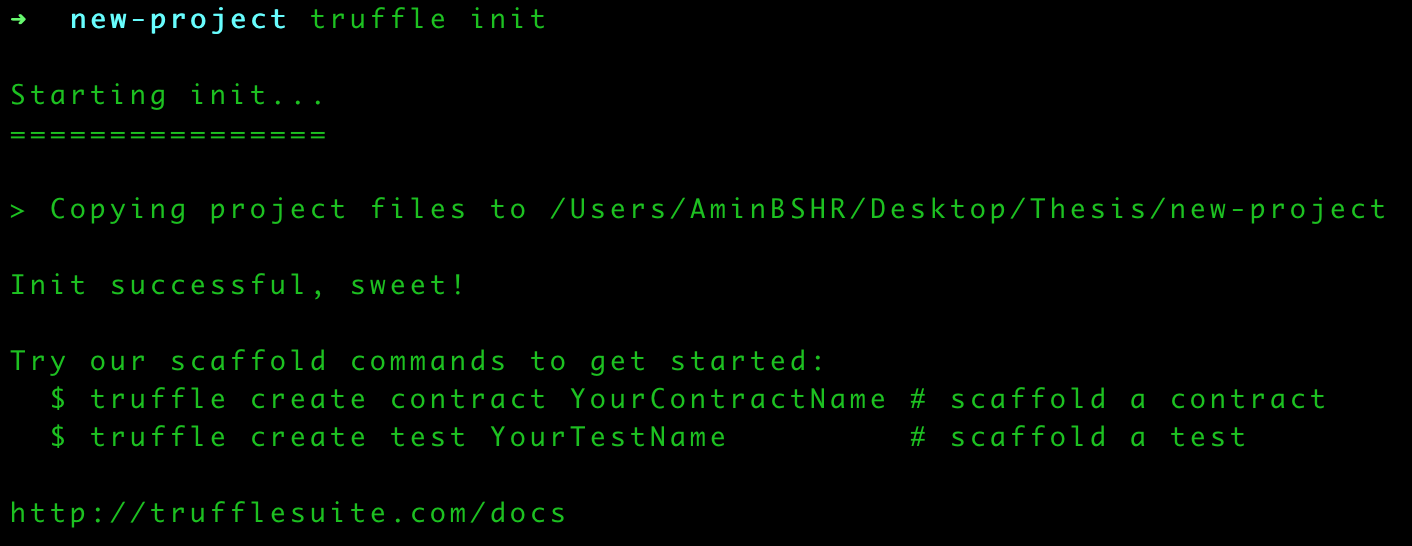
\includegraphics[width=14cm]{truffle-init.png}}}
\caption{اجرای دستور \lr{truffle init}}
\label{fig:truffle-init}
\end{figure}

پس از ساخت پروژه با اجرای دستور
\lr{truffle develop}
مانند تصویر
\ref{fig:truffle-develop}
و یا
\lr{truffle console}
 می‌توان وارد خط فرمان ترافل شد.

\begin{figure}[H]
\centerline{\frame{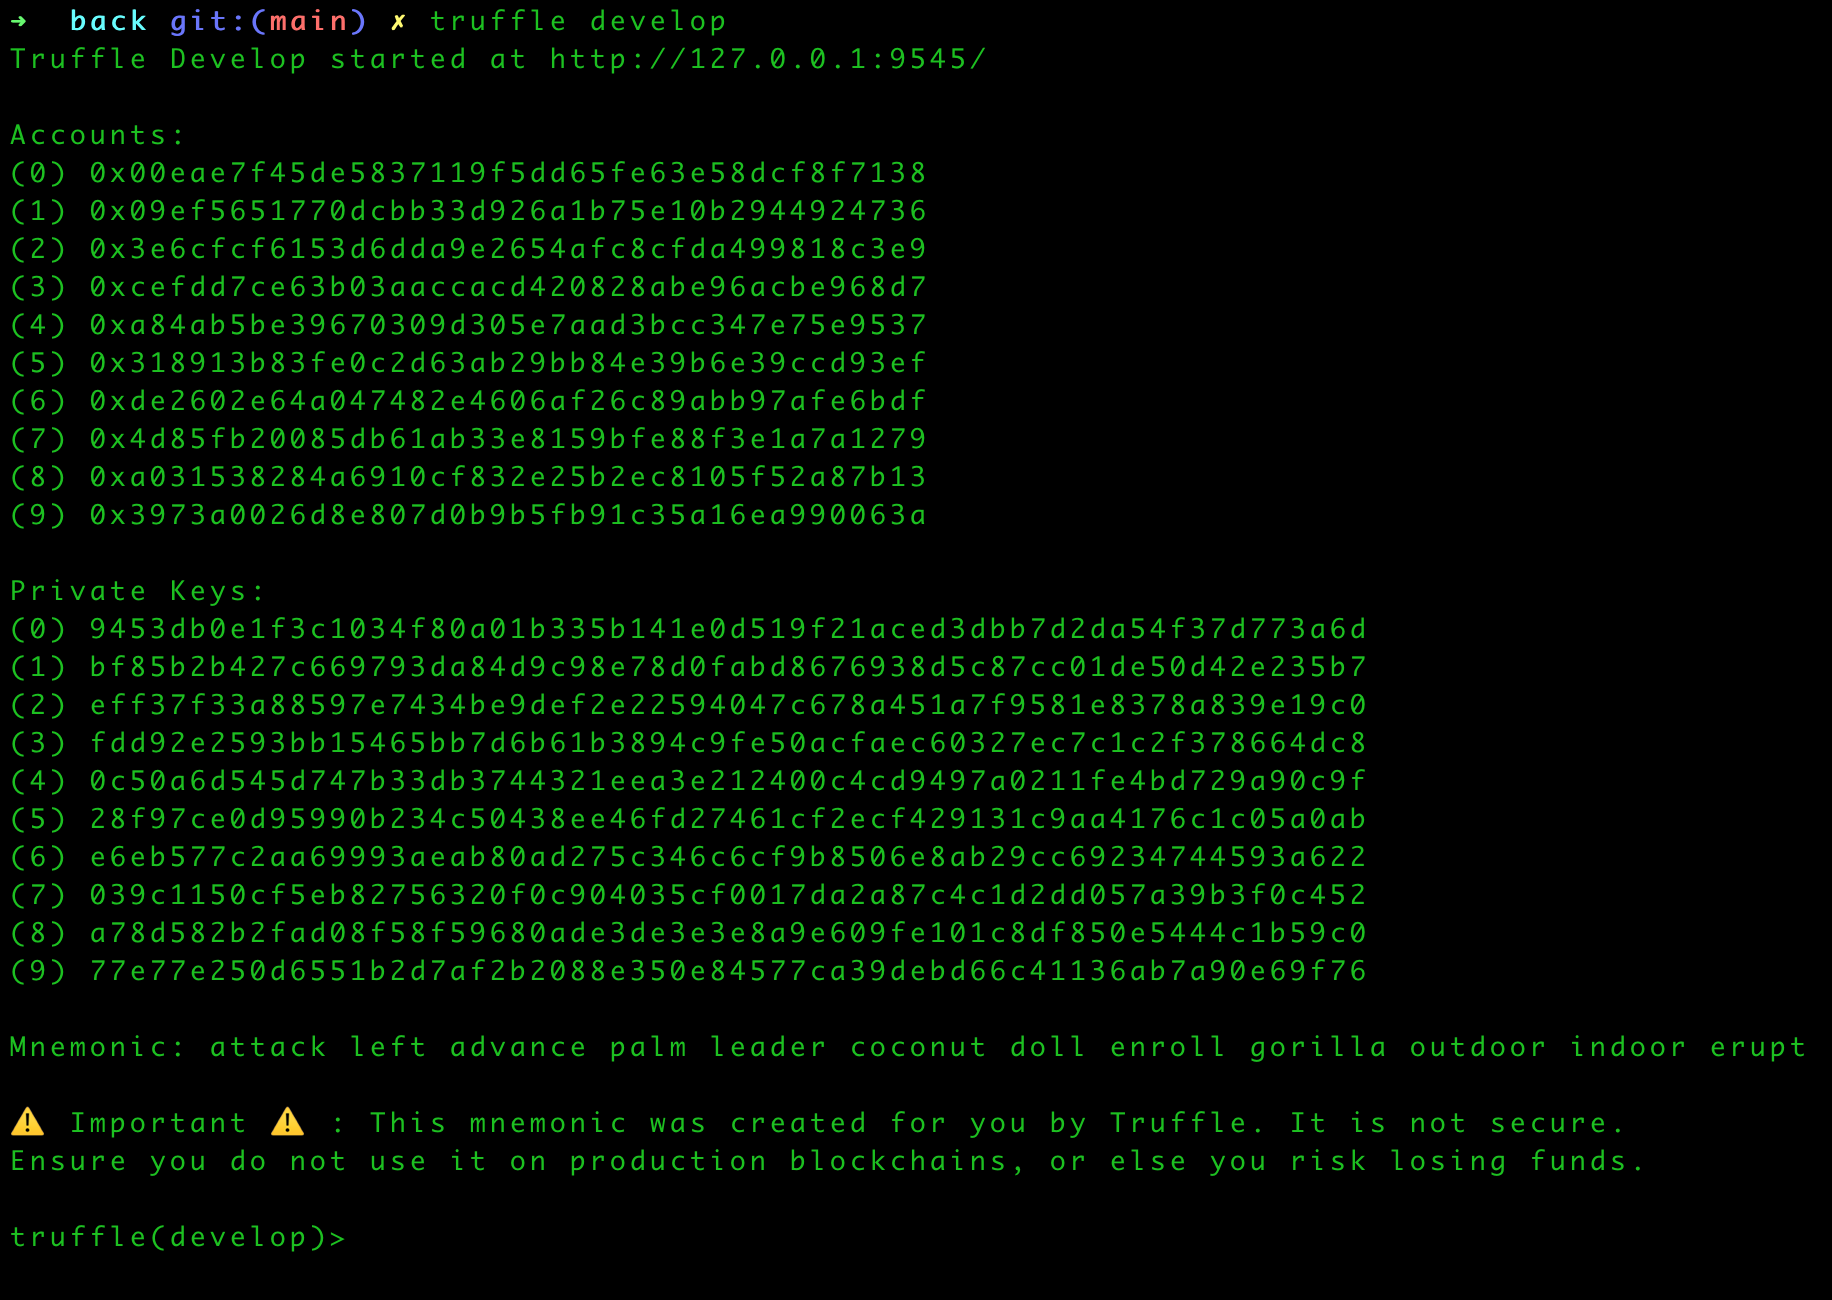
\includegraphics[width=14cm]{truffle-develop.png}}}
\caption{اجرای دستور \lr{truffle develop}}
\label{fig:truffle-develop}
\end{figure}

دستورات لازم برای اجرای آزمون‌ها،
کامپایل کردن قرارداد هوشمند یا بارگذاری آن روی شبکه مورد نظر از طریق این خط فرمان قابل اجرا هستند.
این پلتفرم ابزارهای فراوانی را در اختیار توسعه‌دهنده قرار می‌دهد
که با تعداد بیشتری از آن‌ها در بخش پیاده‌سازی و بارگذاری کاپو آشنا می‌شویم.
همچنین از بزرگترین مزایای استفاده از این چارچوب برقراری ارتباط بسیار آسان با ابزارهای دیگر مانند
\gls{Ganache}
و
\gls{Drizzle}
است.

\subsection{کتابخانه اپن‌زپلین}
یکی از معروف‌ترین کتابخانه‌های قراردادهای هوشمند و استانداردهایشان است.
قراردادها و استانداردهای موجود در این کتابخانه
کاملا آزمون شده، داکیومنت شده، ایمن و پایه بسیاری از قراردادهای هوشمند بر بستر بلاکچین هستند.
استانداردهای ذکر شده در این متن مانند،
\lr{ERC20}،
\lr{ERC721}
و
\lr{ERC1155}
به همراه تعداد زیادی استانداردهای دیگر در این کتابخانه پیاده‌سازی شده‌اند.

در کاپو نیز از استاندارد
\lr{ERC721}
پیاده‌سازی شده در این کتابخانه استفاده شده است.
برای استفاده از قرارداد‌های اپن‌زپلین در قدم اول باید این کتابخانه به کمک دستور
\lr{npm install @openzeppelin/contracts}
نصب شود. پس از نصب کتابخانه، می‌توان از قراردادهای آن ارث‌بری کرد.
در تصویر
\ref{fig:inherit-erc721}
مشاهده می‌شود که کاپو چگونه از قرارداد
\lr{ERC721}
موجود در اپن‌زپلین و همچنین یک قرارداد هوشمند به اسم
\lr{Helper}
که در همین پروژه نوشته شده ارث‌بری کرده است.

\begin{figure}[H]
\centerline{\frame{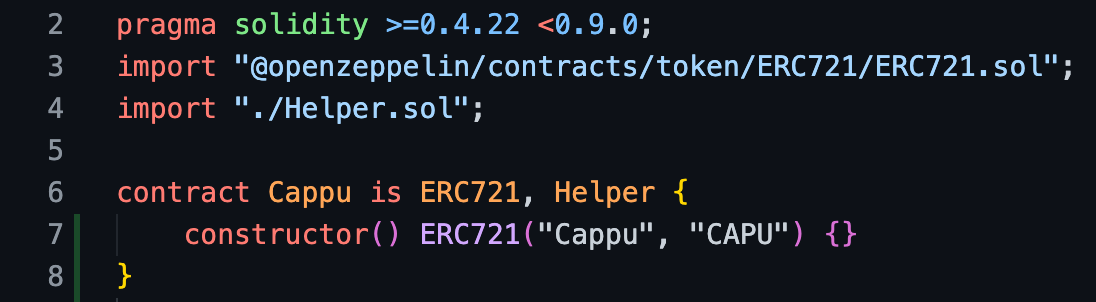
\includegraphics[width=14cm]{inherit-erc721.png}}}
\caption{ارث‌بری از استاندارد \lr{ERC721} پیاده‌سازی شده توسط اپن‌زپلین}
\label{fig:inherit-erc721}
\end{figure}

\subsection{کتابخانه \lr{Web3JS}}
تراکنش‌های با یک قرارداد هوشمند می‌تواند به دو حالت باشد.
در حالت اول فقط اطلاعات شبکه بلاکچین خوانده می‌شود و در
\gls{State}
آن تغییری داده نمی‌شود.
تابع‌های از این جنس از نوع
\lr{view}
یا
\lr{pure}
هستند. حالت دوم تراکنش‌هایی هستند که باعث تغییر اطلاعات شبکه بلاکچین می‌شوند.

واسط‌کاربری یک اپلیکیشن غیرمتمرکز برای انجام نوع اول تراکنش‌ها
نهایتا فقط به آدرس کاربر نیاز دارد
که اطلاعات مربوط به او را از قرارداد دریافت کند.
در حالت دوم نیاز است که تراکنشی بر روی شبکه ثبت شود.
این کار نیازمند امضا شدن تراکنش توسط کلید خصوصی کاربر،
پرداخت کارمزد تراکنش و ارسال آن به نُدهای شبکه است.

کتابخانه‌ی
\lr{Web3JS}
به توسعه‌دهنده کمک می‌کند که واسط‌کاربری اپلیکیشن را به کیف پول دیجیتال کاربر و شبکه بلاکچین متصل کند.
با ایجاد این اتصال آدرس کاربر توسط کیف پول دیجیتال در اختیار واسط‌کاربری قرار می‌گیرد.
هرگاه که واسط‌کاربری بخواهد تراکنشی را روی شبکه ارسال کند نیز از کیف پول کاربر می‌خواهد
که با داشتن کلید خصوصی کاربر آن تراکنش را امضاو روی شبکه ارسال کند.
کیف پول کاربر برای انجام هر یک از این مراحل از کاربر درخواست ثبت تاییدیه می‌کند.


% ------------ Section 3.4
\section{شبکه محلی برای توسعه}
برای توسعه یک قرارداد هوشمند نیاز است
که قرارداد پس از هر تغییر کامپایل و روی یک شبکه بلاکچین بارگذاری شود،
به نحوی که واسط‌کاربری اپلیکیشن و همچنین کیف پول متامسک بتوانند به آن متصل شوند.
از شبکه اصلی نمی‌توان استفاده کرد زیرا هر بارگذاری روی شبکه اصلی هزینه‌ای خواهد داشت
و بارگذاری‌های متعدد روی شبکه اصلی امکان پذیر نخواهد بود.
اگر بخواهیم برای توسعه از شبکه آزمایشی استفاده کنیم نیز
گرچه هزینه‌ای نخواهد داشت اما بسیار زمان‌بر خواهد بود.
ثبت تراکنش‌ها روی شبکه آزمایشی معمولا سریعتر از شبکه اصلی انجام می‌شود
اما همچنان توسعه‌دهنده زمان زیادی را برای هر بارگذاری مصرف خواهد کرد.

راه حل این مشکل این است که توسعه‌دهنده روی ماشین خودش یک شبکه محلی داشته باشد،
که بتواند بلافاصله پس از ایجاد یک تغییر روی قرارداد هوشمند آن را کامپایل و بارگذاری کند.
ترافل باید بتواند به این شبکه محلی متصل شده و قرارداد را روی آن بارگذاری کند.
واسط‌کاربری و متامسک نیز باید بتوانند به این شبکه متصل شوند که با قرارداد هوشمند ارتباط برقرار کنند.

اگرچه ابزارهای زیادی برای ساخت این شبکه محلی وجود دارند،
اما یکی از بهترین و راحت‌ترین ابزارها برای این منظور برنامه‌ی
\gls{Ganache}
هست.
این ابزار با توجه به این که متعلق به اکوسیستم ترافل هست،
به آسانی به آن متصل شده و با اضافه کردن آدرس آن به شبکه‌های متامسک،
این کیف پول نیز به شبکه محلی اتصال می‌یابد.
جزئیات ساخت شبکه محلی و اتصال ترافل و متامسک به آن به ترتیب زیر است.

اگرچه توضیحات کامل نحوه استفاده از گاناچه در مستندات این ابزار
\cite{GanacheDocs}
نیز آمده است، اما در این قسمت توضیحات کوتاه مورد نیاز داده می‌شود.
پس از نصب برنامه گاناچه باید یک
\gls{Workspace}
\gls{Ethereum}
ساخته شود. برای انجام این کار گزینه
\newline
\lr{{New workspace (Ethereum)}}}
انتخاب می‌شود. این دکمه در تصویر
\ref{fig:ganache-1}
قابل مشاهده است.

\begin{figure}[H]
\centerline{\frame{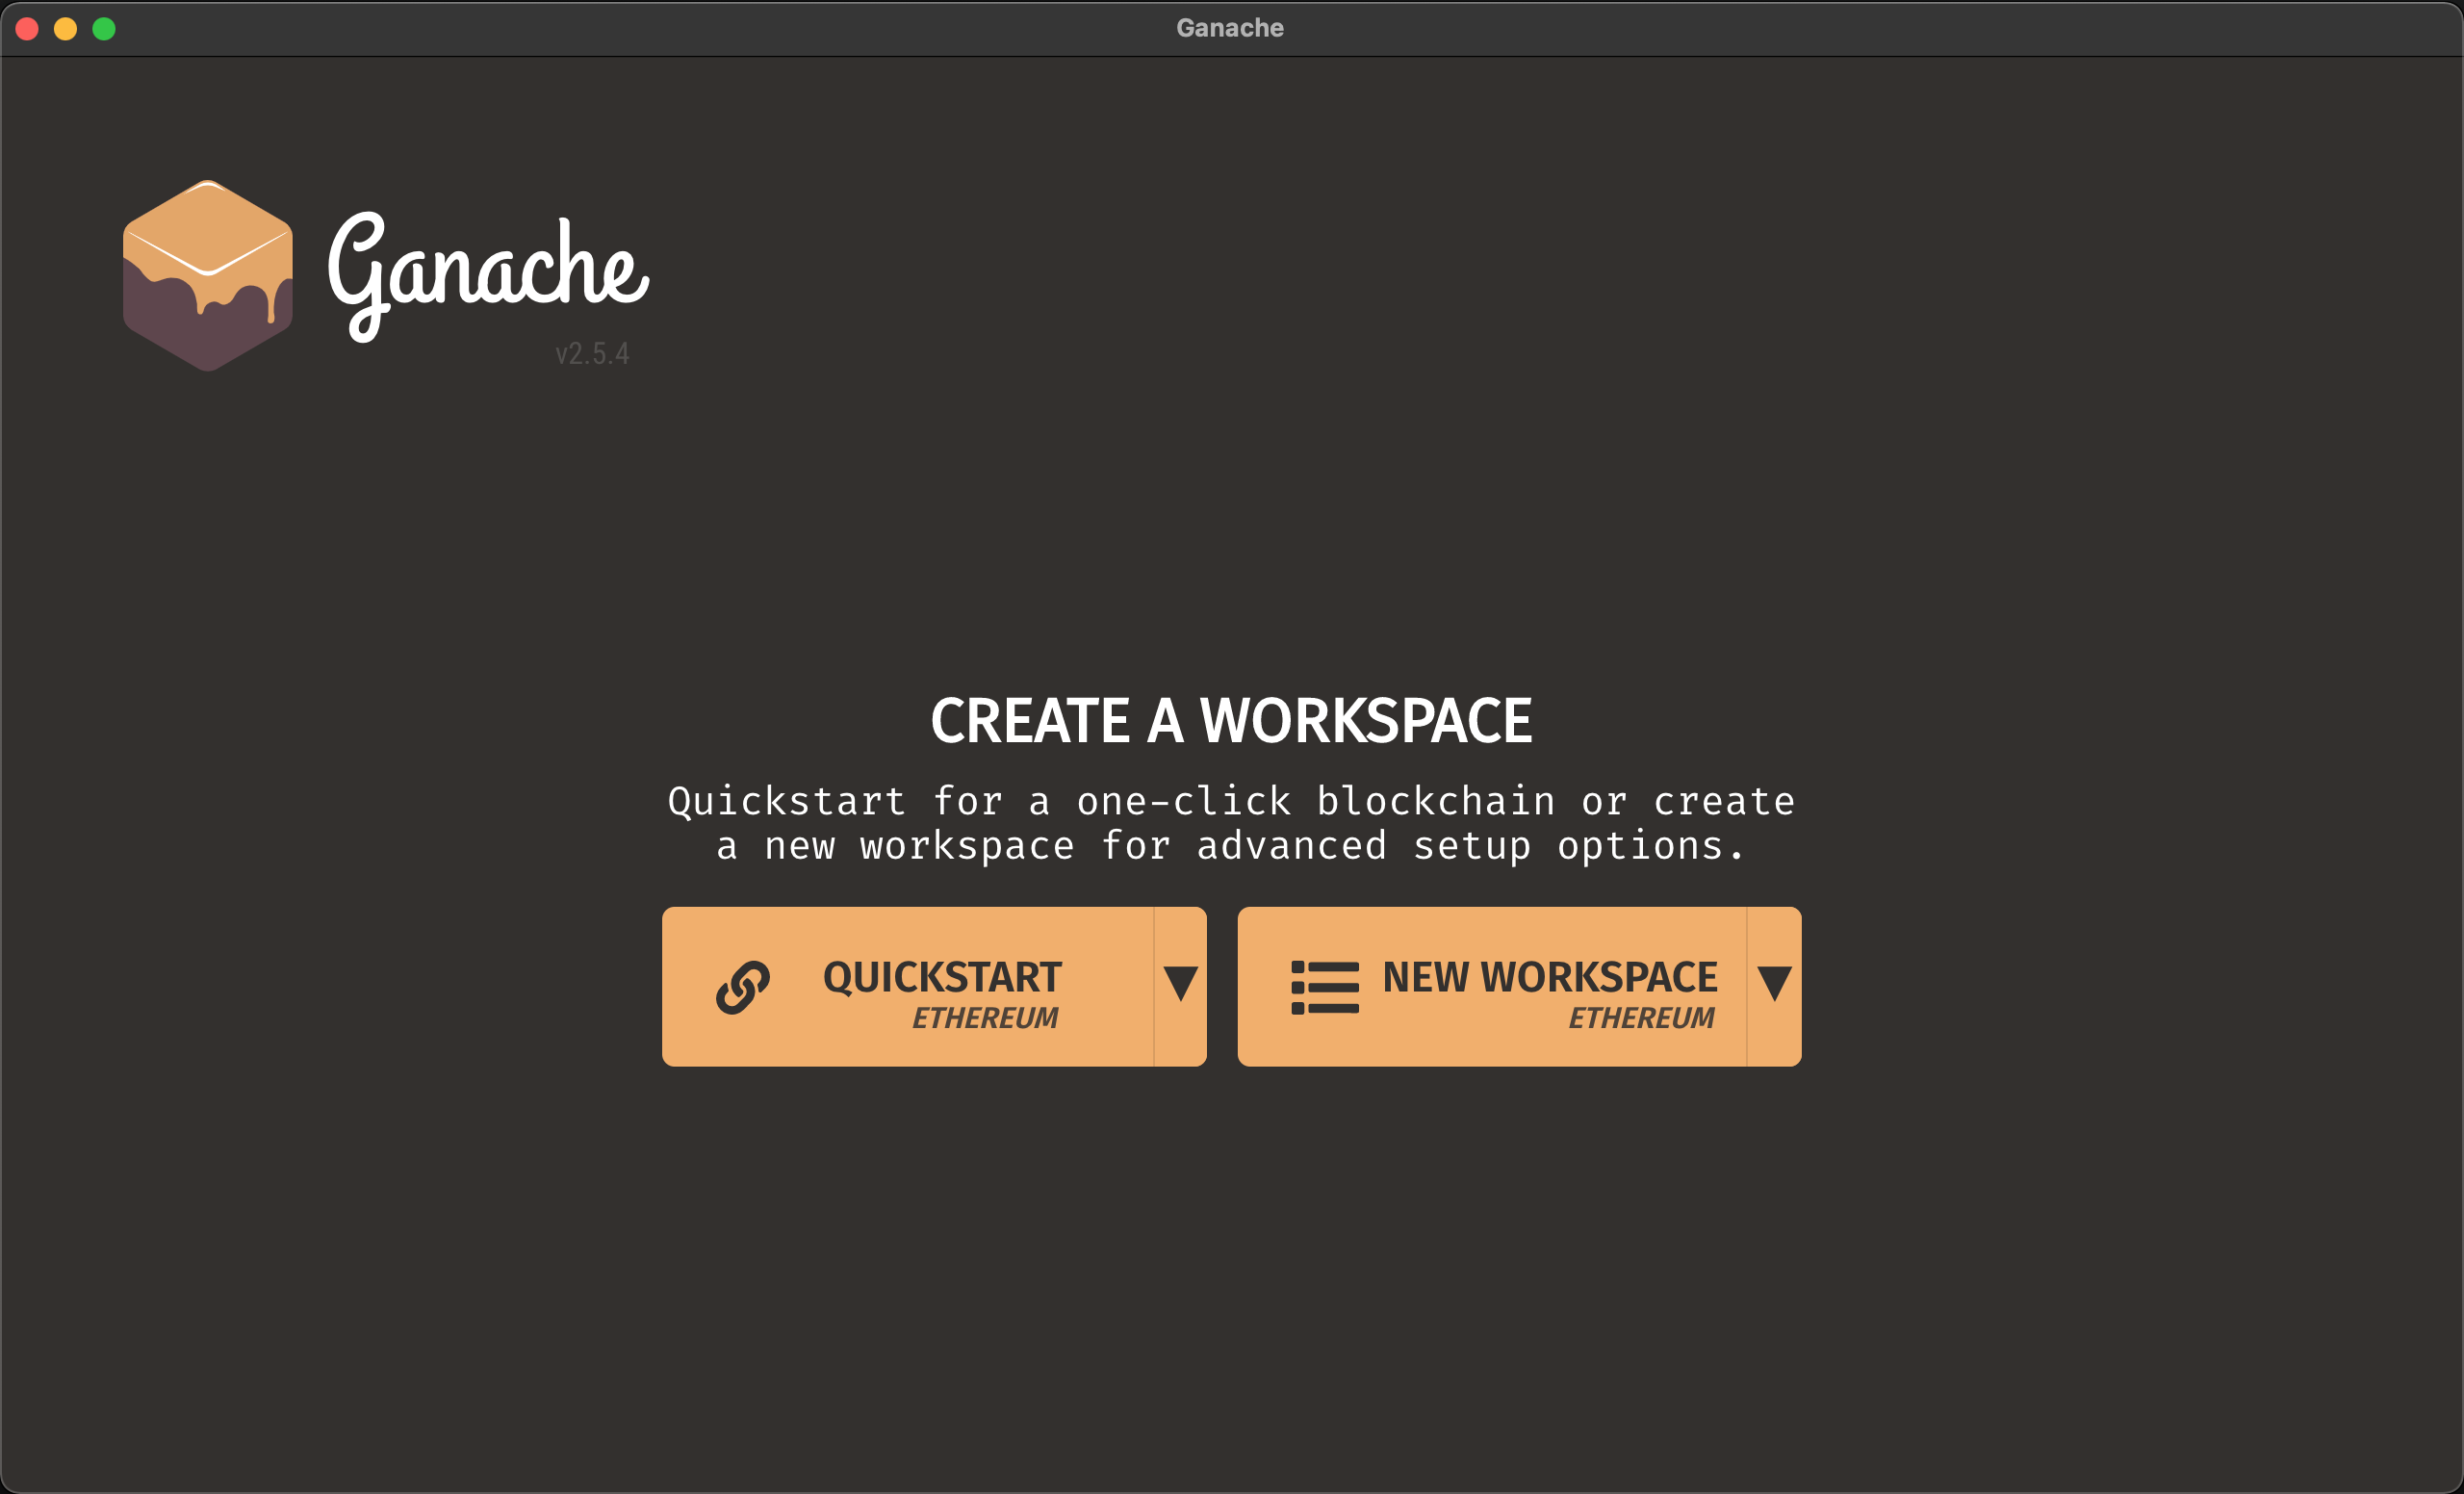
\includegraphics[width=14cm]{ganache-1.png}}}
\caption{صغحه اول گاناچه}
\label{fig:ganache-1}
\end{figure}

سپس در صفحه باز شده نام محیط توسعه وارد،  فایل
\lr{truffle-config.js}
مربوط به پروژه مورد نظر انتخاب و دکمه
\lr{save workspace}
زده می‌شود. انجام این مرحله در تصویر
\ref{fig:ganache-2}
قابل مشاهده است.

\begin{figure}[H]
\centerline{\frame{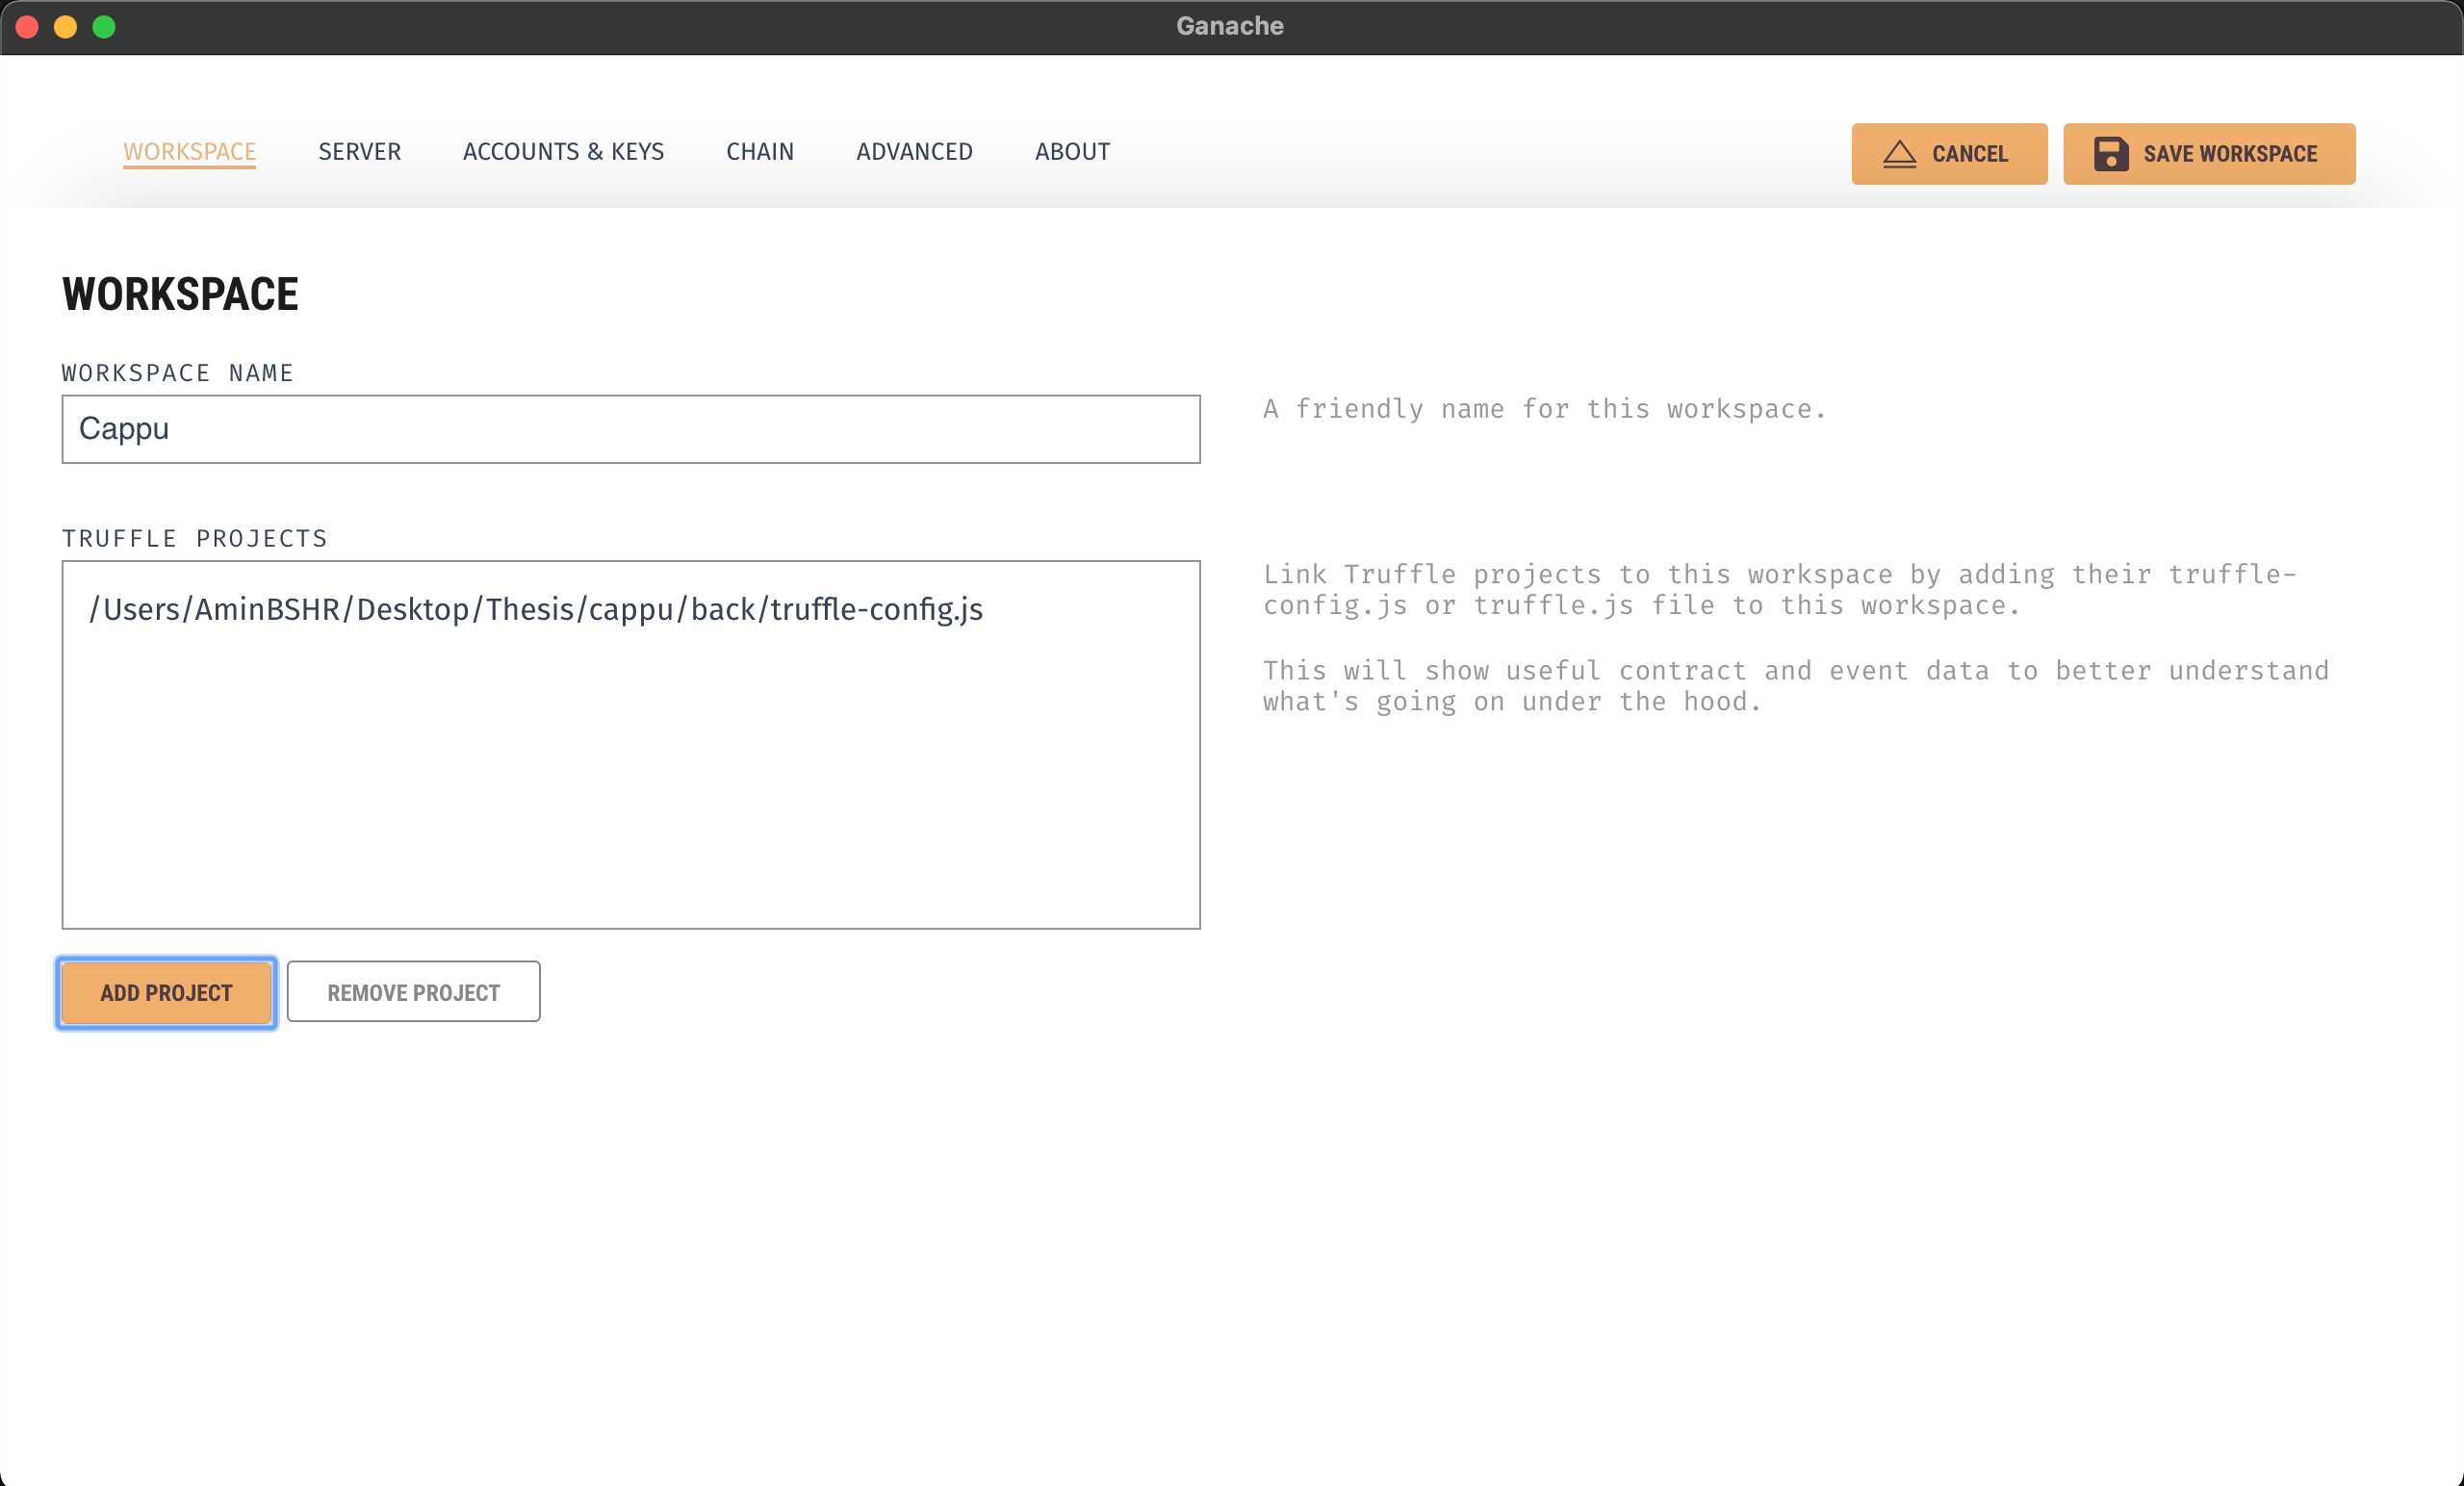
\includegraphics[width=14cm]{ganache-2.png}}}
\caption{ساخت شبکه جدید در گاناچه}
\label{fig:ganache-2}
\end{figure}

پس از انجام این مراحل محیط توسعه ساخته شده است و می‌توان جزئیات شبکه محلی را مشاهده کرد.

\begin{figure}[H]
\centerline{\frame{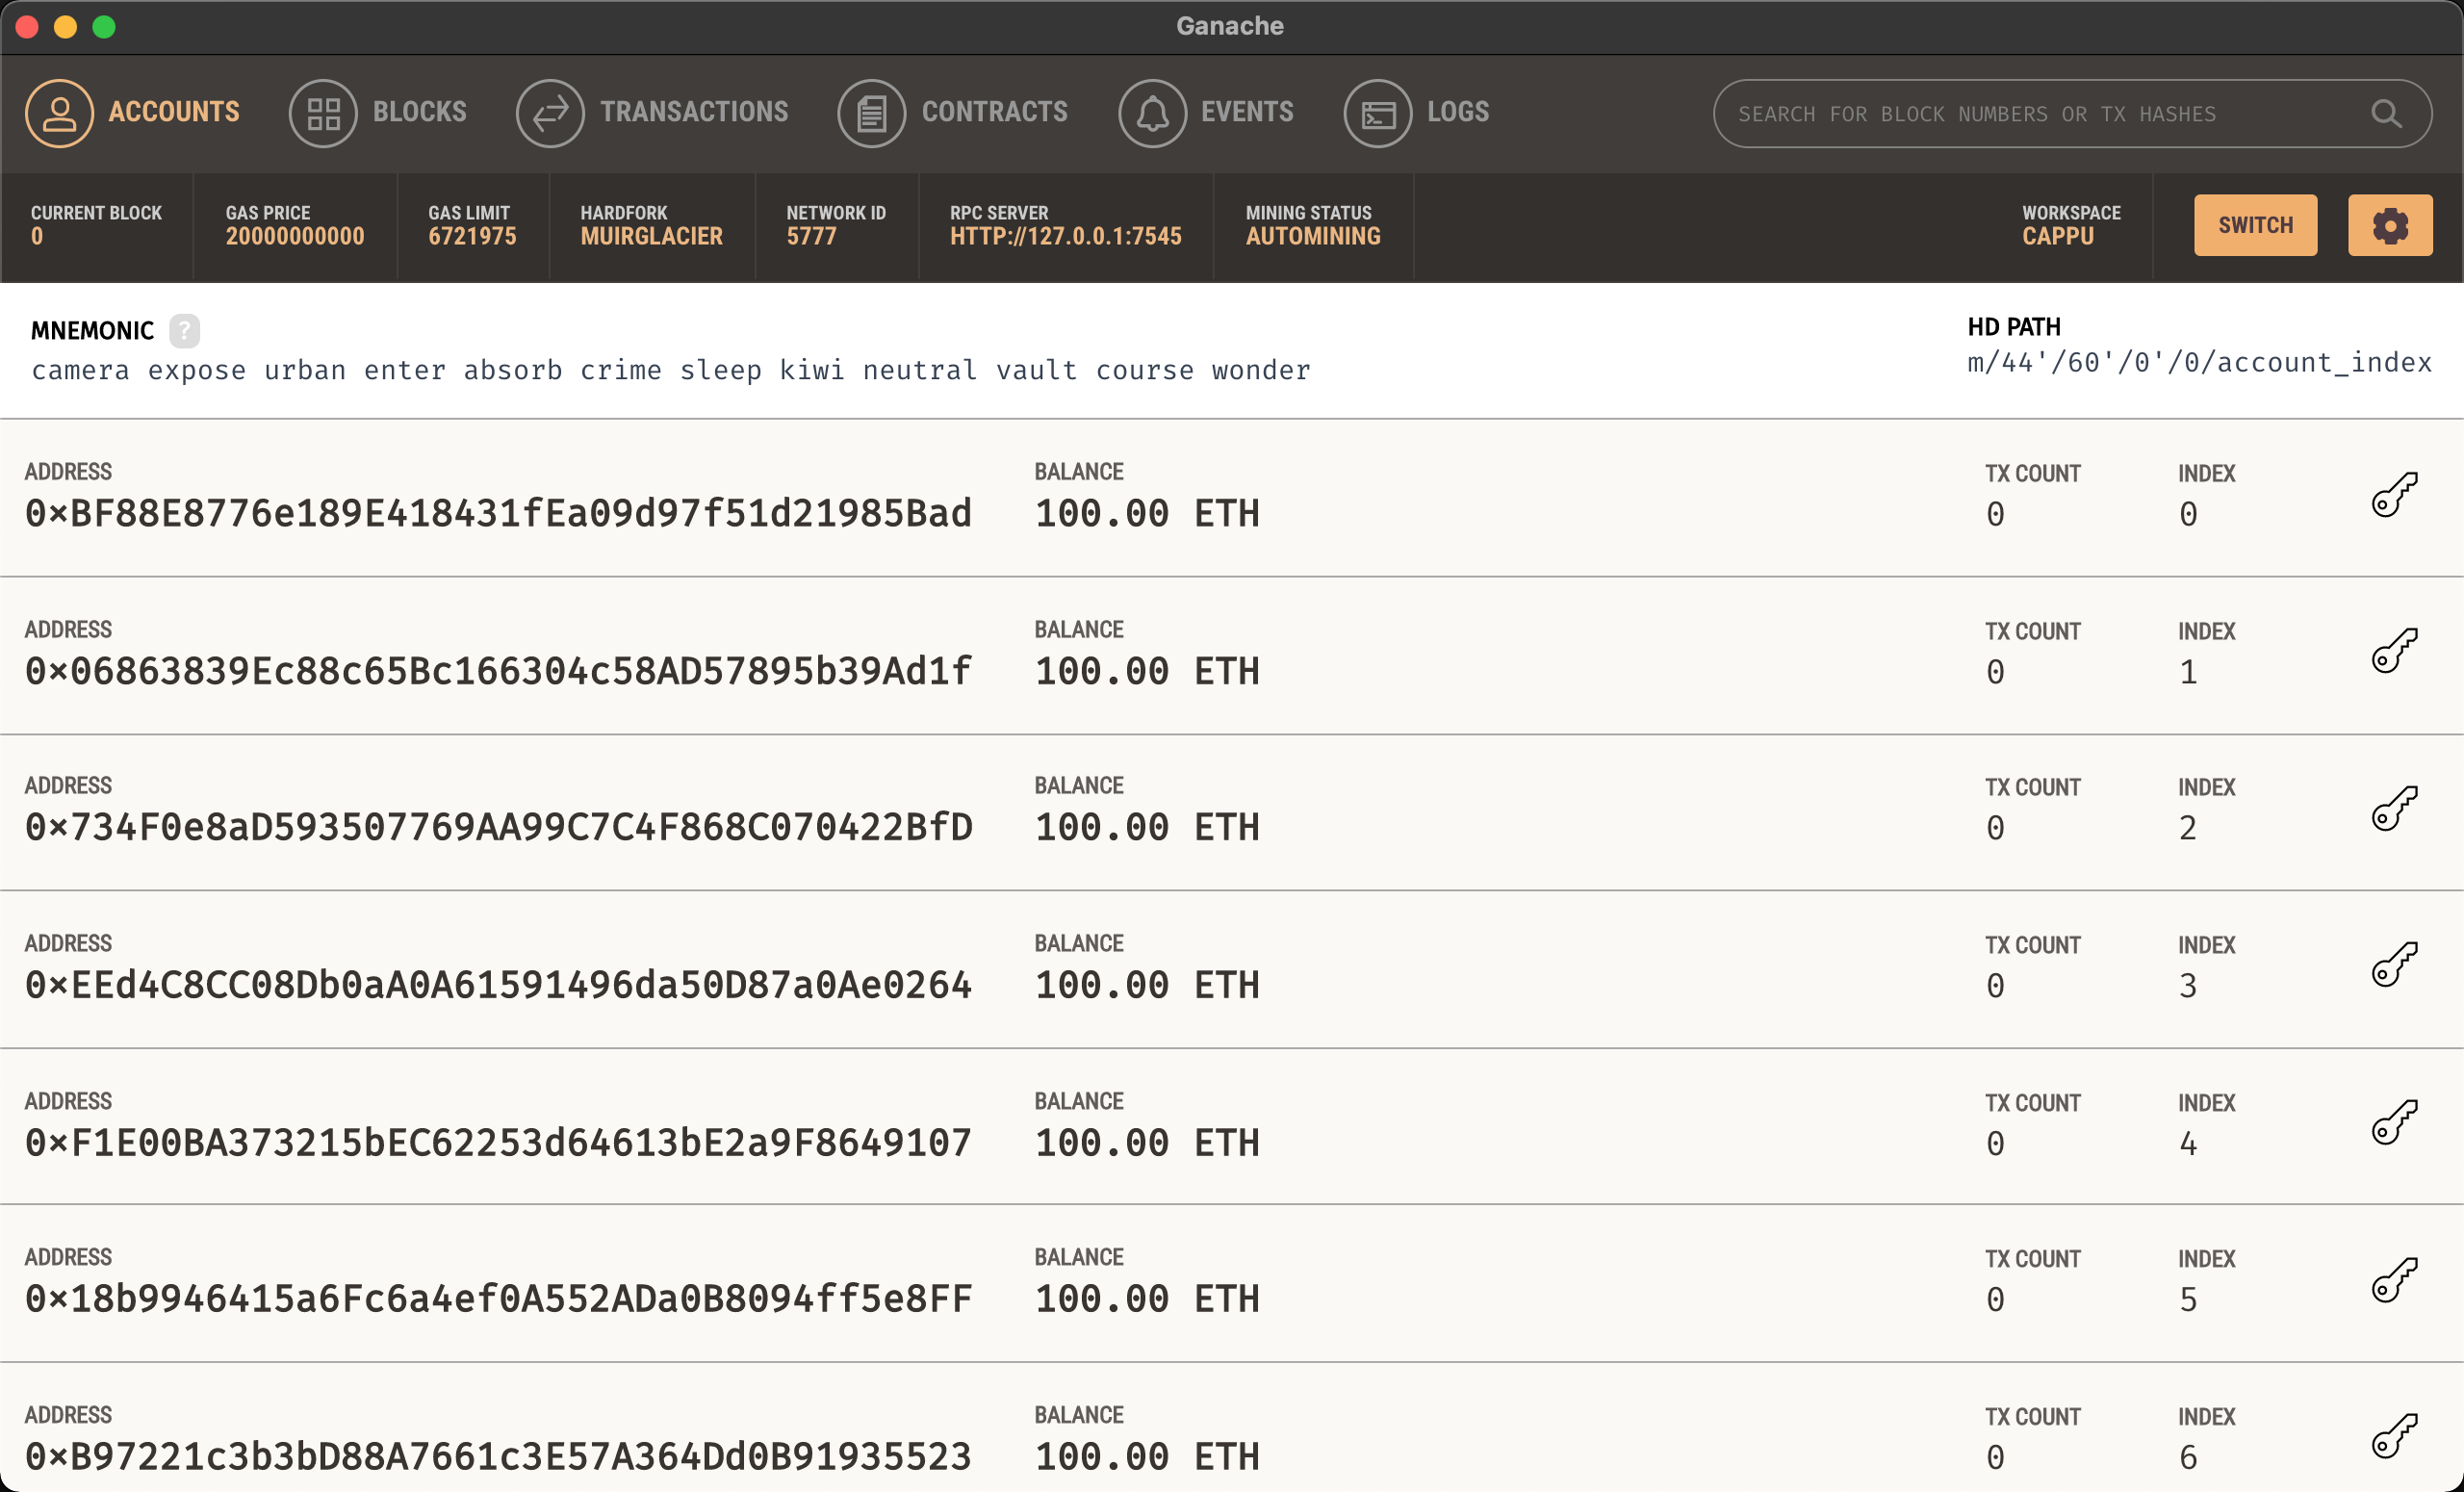
\includegraphics[width=14cm]{ganache-3.png}}}
\caption{مشاهده جزئیات شبکه ساخته شده}
\label{fig:ganache-3}
\end{figure}

از آنجایی که در مرحله قبل برای ساخت این محیط توسعه فایل
\lr{truffle-config.js}
پروژه انتخاب شد، حال اگر دستورات
\lr{truffle console}
یا هر دستور دیگری مانند
\lr{migrate}
بدون انتخاب شبکه بلاکچین خاصی اجرا شود به صورت پیش‌فرض روی این شبکه محلی انجام می‌شود.

حال فقط باید متامسک نیز به این شبکه محلی متصل شود.
برای انجام این کار پس از نصب افزونه‌ی متامسک روی مرورگر کروم، در قسمت
\gls{Settings}
و سپس
\glspl{Network}
یک شبکه جدید مطابق تصویر
\ref{fig:metamask-network}
ساخته می شود، همانطور که در تصویر
\ref{fig:ganache-3}
مشخص است اطلاعات شبکه محلی در صفحه اصلی گاناچه قابل مشاهده هستند.

\begin{figure}[H]
\centerline{\frame{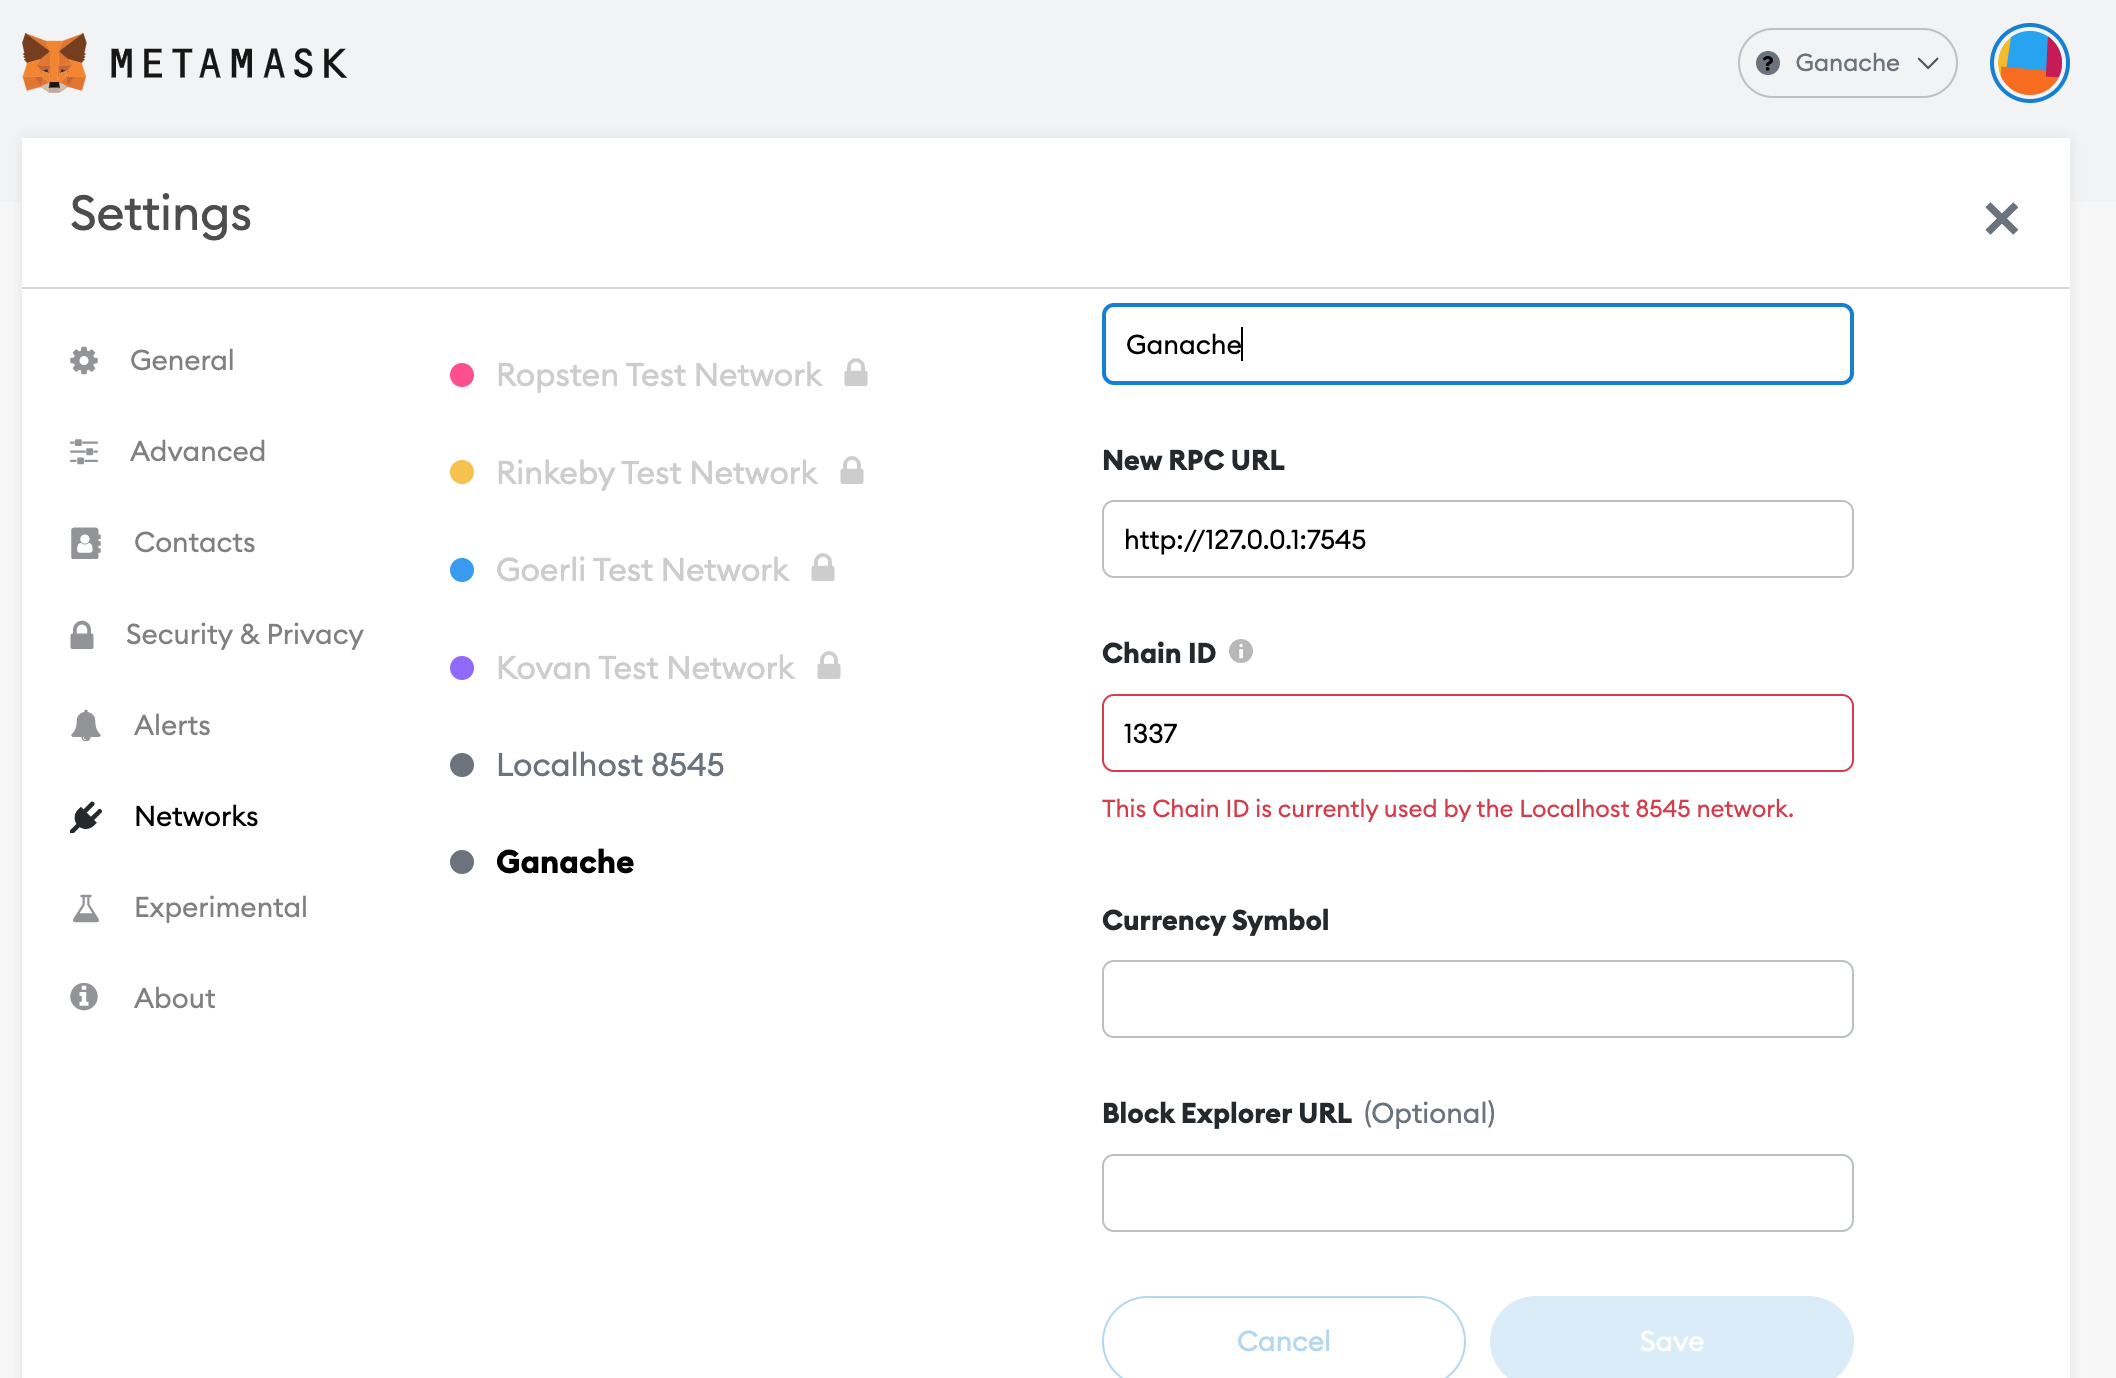
\includegraphics[width=14cm]{metamask-network.png}}}
\caption{تنظیمات شبکه‌های متامسک}
\label{fig:metamask-network}
\end{figure}

پس از ذخیره شبکه جدید کافیست که برای توسعه شبکه گاناچه انتخاب شود.
همچنین باید یکی از آدرس‌هایی که در صفحه اصلی گاناچه نمایش داده می‌شوند به عنوان کیف پول در متامسک وارد شود.
برای انجام این کار علامت کلید کنار یکی از آدرس‌های نمایش داده شده در صفحه اصلی گاناچه انتخاب می‌شود
و به کمک کلید اختصاصی نمایش داده شده کیف پول در متامسک وارد می شود.
